\chapter{Implementation}
 \section{Installation and Configuration of the surroundings}
  \subsection{Installation}
  \label{sec:implementation:installation}
   To install the Software project management system (see section \ref{sec:research:softwareProjectManagement}) with Subversion (see section \ref{sec:research:codeVersionControl}) connection, the following packages need to get installed on the server:
   \begin{itemize}
    \item apache
    \item subversion
    \item trac
    \item phpMyAdmin
   \end{itemize}

  \subsection{Configuration}
   The following sections cover the basic configurations for the project surroundings. The base name for the system is dld (domestic location detection) and therefore it will be used for the subversion repository and trac.

   \subsubsection{Subversion}
    To use a subversion code version control system with this project, the project needs a repository. The command to do this is:\\
    \verb=svnadmin create /var/svn/dld=
    
    After the repository is created the permissions have to be set such that the apache webserver gets access to the repository as well. Therefore we create a new group called \verb=svnusers=, adding the apache to this group and changing the permissions of the repository directory:
    \begin{enumerate}
     \item groupadd svnusers
     \item usermod -G svnusers -a apache
     \item chgrp svnusers /var/svn/dld -R
     \item chmod g+w /var/svn/dld -R
    \end{enumerate}

   \subsubsection{trac}
    To configure trac the base system needs to be installed to the directory where the web pages are stored. On gentoo this is done by the following command:\\
    \verb=webapp-config -I -d dld/trac trac 0.10.3.1=

    Assuming that 0.10.3.1 is the current version of the trac package, if not then it needs to be replaced by the current version. To initially configure trac the administrator just has to use the administration tool that comes with the trac package. The following shows how to execute it:\\
    \verb=trac-admin /var/lib/trac/dld initenv=

    The program then asks for a few details and afterwards it installs the files to the directory that was given to the \verb=webapp-config= program.

    After the basic configuration is done the trac system needs to be cleaned from previous made example entries. In addition to that, a few changes need to be done to the permissions of the anonymous user and a whole new user(in this case the developer) should be added who has the right to change everything on the system. To enter the interactive control console for trac the administrator needs to execute the following command:\\
    \verb=trac-admin /var/lib/trac/dld=

    \begin{lstlisting}[frame=single,breaklines,basicstyle=\footnotesize,numbers=left,label=lst:tracCleanUpCommands,captionpos=b,caption={clean up command for the trac administration console}]
milestone remove milestone1
milestone remove milestone2
milestone remove milestone3
milestone remove milestone4
milestone remove milestone1
milestone remove milestone2
milestone remove milestone3
milestone remove milestone4
version remove 1.0
version remove 2.0
component remove component1
component remove component2
permission remove anonymous WIKI_MODIFY WIKI_CREATE
permission add twist BROWSER_VIEW CHANGESET_VIEW CONFIG_VIEW FILE_VIEW LOG_VIEW MILESTONE_ADMIN MILESTONE_CREATE MILESTONE_DELETE MILESTONE_MODIFY MILESTONE_VIEW REPORT_ADMIN REPORT_CREATE REPORT_DELETE REPORT_MODIFY REPORT_SQL_VIEW REPORT_VIEW ROADMAP_ADMIN ROADMAP_VIEW SEARCH_VIEW TICKET_ADMIN TICKET_APPEND TICKET_CHGPROP TICKET_CREATE TICKET_MODIFY  TICKET_VIEW TIMELINE_VIEW TRAC_ADMIN WIKI_ADMIN WIKI_CREATE WIKI_DELETE WIKI_MODIFY WIKI_VIEW
    \end{lstlisting}
    Listing \ref{lst:tracCleanUpCommands} shows the commands that need to be entered to remove all unnecessary entries and to change the permissions. The user \verb=twist= will be used by the developer as a nickname to the system.

   \subsubsection{Apache}
   First we create a password file that will be used for authorisation of the developers both through the trac interface and to authorise them to be able to commit changes to the repository.\\
   \verb=htpasswd2 -c /etc/apache2/trac.htpasswd twist=

   After this is done the files /etc/apache2/vhosts.d/00\_default\_vhost.conf and /etc/apache2/modules.d/99\_trac.conf needs to be adjusted. The \dots/99\_trac.conf has to look like the one in listing \ref{lst:adjustment99trac} and the lines from listing \ref{lst:adjustment00DefaultVhost} have to be added to the \verb=<VirtualHost *:80>= section of the \dots/00\_default\_vhost.conf file.

   \begin{lstlisting}[frame=single,breaklines,basicstyle=\footnotesize,numbers=left,label=lst:adjustment99trac,captionpos=b,caption={Adjustment of the file /etc/apache2/modules.d/99\_trac.conf}]
ScriptAlias /dld/trac /var/www/localhost/cgi-bin/trac.cgi
# This location should match the ScriptAlias above, if you want trac
# to be hosted at http://localhost/projects instead of http://localhost/trac
# change both the ScriptAlias and the Location.
<Location "/dld/trac">
	SetEnv TRAC_ENV "/var/lib/trac/dld"
	# Comment TRAC_ENV above and uncomment TRAC_ENV_PARENT_DIR
	# below to enable one Trac installation to handle multiple
	# Trac projects
	#SetEnv TRAC_ENV_PARENT_DIR "/var/lib/trac/"
</Location>
# Configure how Trac will authenticate users
<Location "/cgi-bin/trac.cgi/login">
	# Using htpasswd for authentication
	AuthType Basic
	AuthName "trac"
	# Create an htpasswd file for trac users and
	# reference it here:
	AuthUserFile /etc/apache2/trac.htpasswd
	Require valid-user
</Location>
   \end{lstlisting}

   \begin{lstlisting}[frame=single,breaklines,basicstyle=\footnotesize,numbers=left,label=lst:adjustment00DefaultVhost,captionpos=b,caption={Adjustment of the file /etc/apache2/vhosts.d/00\_default\_vhost.conf}]
# dld - trac
	Alias /dld/dox /var/www/localhost/htdocs/dld/dox
	<Location /dld/svn>
		<IfDefine SVN>
			DAV svn
			SVNPath /var/svn/dld
			SVNIndexXSLT /dld/trac/svnindex.xsl
		</IfDefine>
		<LimitExcept GET PROPFIND OPTIONS REPORT>
			AuthType Basic
			AuthName "DLD::svn"
			AuthUserFile /etc/apache2/trac.htpasswd
			Require valid-user
		</LimitExcept>
	</Location>
	<Location /dld>
		SetEnv TRAC_ENV "/var/lib/trac/dld"
	</Location>
	# Configure how Trac will authenticate users
	<Location /dld/login>
		AuthType Basic
		AuthName "DLD::trac"
		AuthUserFile /etc/apache2/trac.htpasswd
		Require valid-user
	</Location>
	Alias /dld/trac /var/www/localhost/htdocs/dld/trac
	ScriptAlias /dld /var/www/localhost/cgi-bin/trac.cgi
# dld - trac - end
   \end{lstlisting}

  \subsection{Adding the basic directory structure to the Subversion repository}
   For adding the basic structure it needs to be created first. To achieve this the project directories will look similar to the modules that were created back in section \ref{sec:design:modularisation} all on top of the three main directories which are commonly used by subversion:
   \begin{lstlisting}[frame=single,breaklines,basicstyle=\footnotesize,numbers=left,label=lst:subversionPaths,captionpos=b,caption={Tree structure of the project in the repository}]
./code/branches/
./code/tags/
./code/trunk/
./code/trunk/dld/src/common
./code/trunk/dld/src/gainData
./code/trunk/dld/src/obConfig
./code/trunk/dld/src/mapGen
./code/trunk/dld/src/generatePosition
./code/trunk/dld/src/showPos
./code/trunk/dld/src/pdAdmin
./code/trunk/dld/doc/
   \end{lstlisting}

   The tree structure described in listing \ref{lst:subversionPaths} needs to be created on the server and after creation it will be imported to the subversion repository with the following command (executed from the directory where the code directory is located, but the code directory will not be part of the repository):\\
   \verb=svn import ./code/ file:///var/svn/dld/=

   After that the code can be fetched from anywhere (with the anonymous account) with the following command:\\
   \verb=svn checkout http://sirtwist.homeip.net/dld/svn=

   Committing source is restricted to the developer therefore the developer needs an other command line to firstly fetch the source code:\\
   \verb=svn checkout http://twist@sirtwist.homeip.net/dld/svn=

   Both the developer fetch of the source code and the anonymous one can both stay up to date with the\\
   \verb=svn update= \\
   command.

  \subsection{Database and phpMyAdmin}
   Like written in the webserver (\ref{sec:research:webServer}) and the database (\ref{sec:research:databases}) section of the Research stage, this project will make use of the apache web server and the mysql database. The database will be administrated with the phpMyAdmin (\url{http://www.phpmyadmin.net/}) interface. The basic installation on modern Linux systems is fairly easy, the packages just needed to be installed through the distribution package system. If the distribution does not provide those packages then the sources can be downloaded and compiled by the developer himself.

  After installing all three components (the apache, the mysql database and the phpMyAdmin) the apache is running out of the box with a default start page. The configuration files of the apache are located in /etc/apache2. The DocumentRoot entry of the configuration file (e.g. /etc/apache2/vhosts.d/default\_vhost.include) specifies where the web pages are stored. The phpMyAdmin interface will be found in that directory. MySQL on the other hand needs some basic configuration:\\

  \begin{lstlisting}[frame=single,numbers=left,basicstyle=\footnotesize,label=lst:mysqlBasicConfigGentoo,captionpos=b,caption={Basic MySQL configuration in Gentoo}]
emerge --config dev-db/mysql
/etc/init.d/mysql start
mysql_setpermission
mysql_secure_installation 
  \end{lstlisting}

  The above listing \ref{lst:mysqlBasicConfigGentoo} shows the basic steps to configure mysql after it was installed. In line one the basic configuration for mysql will be done. Line two starts the mysql server. In line three a shell script is used to help adding, changing and deleting users and databases. The fourth line is optional and will just make sure that insecure elements are removed from the installation (like the anonymous user, forcing a root password and setting permissions).

  After the basic configuration of the MySQL database the phpMyAdmin needs to be configured to communicate with the database. This is done after the apache and mysql servers are started. The phpMyAdmin configuration is done with the web interface.

  \begin{figure}[h]
   \centering
   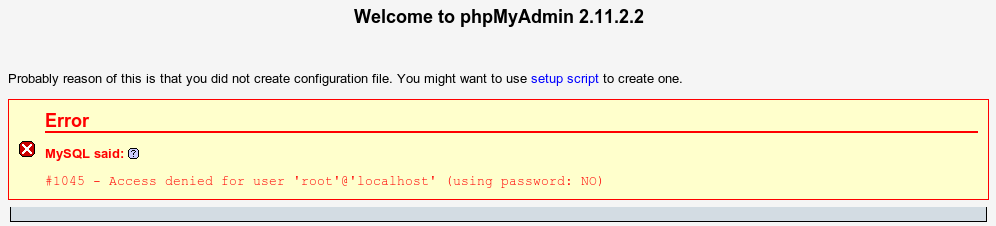
\includegraphics[scale=0.55]{images/ScreenShot-phpMyAdmin-startConfig.png}
   \caption{First start of phpMyAdmin}
   \label{fg:implementation:phpMyAdminConfig:Start}
  \end{figure}

  Figure \ref{fg:implementation:phpMyAdminConfig:Start} shows the page that will come up at the first start of an unconfigured phpMyAdmin interface when typing in the web address \url{http://localhost/phpmyadmin/} regarding that apache and phpMyAdmin are installed on the local machine. If not, localhost needs to be replaced by the appropriate address. The configuration then will start with a click on the setup script button. After the configuration (follow the instructions), phpMyAdmin will present a login dialog under the same address as above. After The login a screen similar to figure \ref{fg:implementation:phpMyAdminConfig:Interface} is shown.

  \begin{figure}[h]
   \centering
   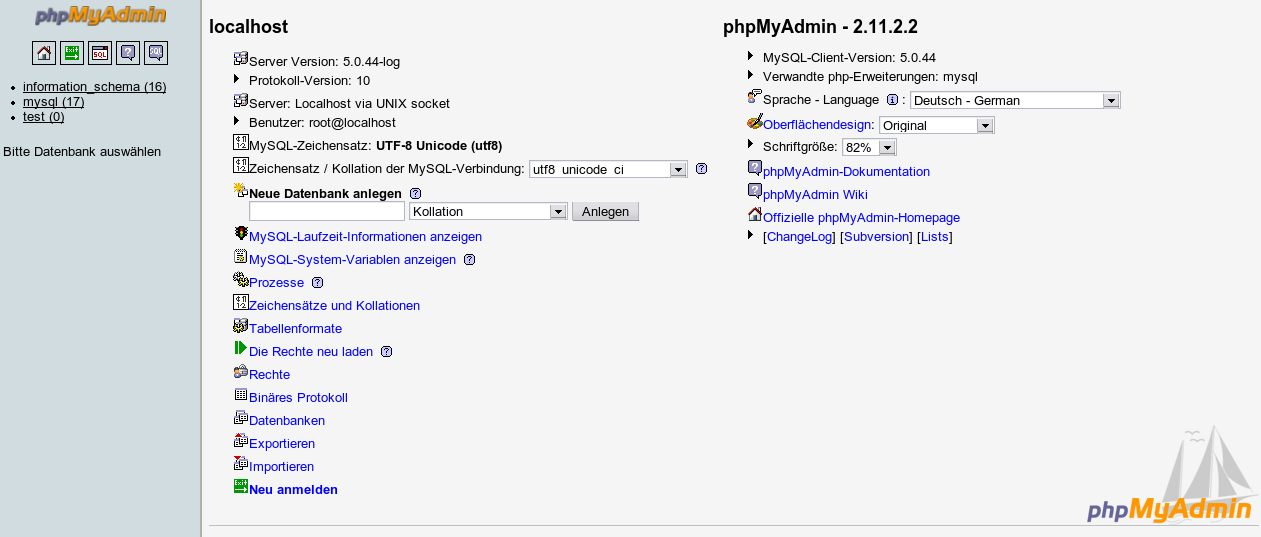
\includegraphics[scale=0.45]{images/ScreenShot-phpMyAdmin.png}
   \caption{phpMyAdmin MySQL interface}
   \label{fg:implementation:phpMyAdminConfig:Interface}
  \end{figure}

  The phpMyAdmin interface of MySQL is very intuitive and helps creating users, tables and databases. Even people who do not know the SQL commands, have the possibility to add, change and edit things.

% END configuration section

 \section{Coding style}
  The coding style should be well defined so everybody who wants to commit source knows in which style it should be sent in. To have a standard is the best way to keep the source in general readable.

  \begin{itemize}
   \item All the implementation is in the .cpp (source) files
   \item All the declarations are in the .h (header) files
   \item The code should be indented with tabs.
   \item A doxygen documentation on top of each function
   \item Comments on difficult source positions should describe what the source is meant to do
   \item Class names start with an uppercased letter
   \item Method names start with a lowercased letter
   \item Globals are complete uppercase
   \item Class, method and variable names should be easy to read or it should be easy to guess what they are for.
   \item Place the brace indented under the statement. Listing \ref{lst:braceIndentExample} shows an example.\\
    \begin{lstlisting}[frame=single,language=C++,breaklines,basicstyle=\footnotesize,numbers=left,label=lst:braceIndentExample,captionpos=b,caption={Example of right placement of braces}]
if (x == 1)
{
	...
}
    \end{lstlisting}
   \item All if, while, for statements require braces even if they only have one statement in between those braces
   \item Class names start with an uppercase letter, while method names start with a lower case one.
  \end{itemize}

 \section{Milestones}
  This section is about the milstones that were reached during the project.

  \subsection{OpenBeacon Configurator + helper classes}
   The first Milestone corresponds to the finalization of the first application which will be the OpenBeacon Configurator. This application will be used to configure the OpenBeacon devices for the project. Additional to the application some common classes will be programmed and tested as well. Those common classes are the ``DLD Log'' class and the ``OpenBeacon Communication'' class. Both classes will be heavily used during the project. Thus a small application which utilizes them is perfect for testing and tuning them.

   The implementation of the application went realy straight forward. First the GUI was designed with the designer application, that comes with the Qt package. After the GUI design was done the functionalities were added step by step.

  \subsubsection*{Problems that occured during the development}
   The OpenBeacon communicator class was planned to be a helper class and only the data gain daemon should have a threaded version of the class. But during the implementation it shows that a threaded version is in need for every application that has to communicate with the openbeacon. Therefore the threaded version planned for the gain data daemon was moved to the OpenBeacon Communication class and thats the reason why the gain data daemon now has less classes to implement and there has more work been done during the implementation of the OpenBeacon Configurator

  \subsection{Firmware}
   To setup the environment for developing the compiler needs to be installed. To do so it needs to be downloaded from the OpenBeacon project via the following URL, \url{http://people.openpcd.org/meri/gnuarm-4.0.2.tar.bz2}. After the download is finished it needs to be unpacked to the root directory.

   This project needs only a few additions to the currently available firmware so now we have to download and unpack the current version and add it to the repository. The needed firmware is the estimator version 008 which can be retrieved from \url{http://www.openbeacon.org/dl/OpenBeacon/estimator-008.tar.bz2}.

   Now the \verb=Makefile= needs some adjustments to use the compilers from the correct destination. On top of the Makefile there are a few variables that have to get changed from:
   \begin{lstlisting}[frame=single,breaklines,basicstyle=\footnotesize,numbers=left,label=lst:firmwareMakefileOld,captionpos=b,caption={Original head of the firmware Makefile}]
CC=arm-elf-gcc
OBJCOPY=arm-elf-objcopy
OBJDUMP=arm-elf-objdump
ARCH=arm-elf-ar
   \end{lstlisting}
   to:
   \begin{lstlisting}[frame=single,breaklines,basicstyle=\footnotesize,numbers=left,label=lst:firmwareMakefileNew,captionpos=b,caption={Changed head of the firmware Makefile}]
CC=/usr/local/gnuarm-4.0.2/bin/arm-elf-gcc
OBJCOPY=/usr/local/gnuarm-4.0.2/bin/arm-elf-objcopy
OBJDUMP=/usr/local/gnuarm-4.0.2/bin/arm-elf-objdump
ARCH=/usr/local/gnuarm-4.0.2/bin/arm-elf-ar
   \end{lstlisting}

   The function that needs to be advanced is \texttt{void prvExecCommand (u\_int32\_t cmd, portCHAR * args)} which can be found in the \verb=application/cmd.c=.

   \begin{center}
    \begin{tabular}{|c|l|}
     \hline
      Function character	& Function description \\
     \hline
     \hline
      D & get the configured Id\\
      M & get the configured mode (returns 0-4) \\
      U & get the uptime in seconds \\
      A & get the channel of the node \\
      L & get FIFO cache lifetime\\
     \hline
    \end{tabular}
   \end{center}

   \subsubsection*{Code changes that were made}
    The only performed changes were done in the file which concerns on the commands: \verb=application/cmd.c=. The switch-case structure was enhanced by the following lines:
    \begin{lstlisting}[frame=single,breaklines,basicstyle=\footnotesize,numbers=left,label=lst:firmwareExtendedCommands,captionpos=b,caption={inserted source to application/cmd.c}]
// below new stuff for FYP from Simon Schaefer
case 'D':
	DumpStringToUSB("Id: ");
	DumpUIntToUSB(env.e.reader_id);
	DumpStringToUSB("\n\r");
	break;
case 'M':
	DumpStringToUSB("Mode: ");
	DumpUIntToUSB(env.e.mode);
	DumpStringToUSB("\n\r");
	break;
case 'U':
	DumpStringToUSB("Uptime: ");
	s=xTaskGetTickCount()/1000;
	DumpUIntToUSB(s);
	DumpStringToUSB("\n\r");
	break;
case 'A':
	DumpStringToUSB("Channel: ");
	DumpUIntToUSB(nRFAPI_GetChannel());
	DumpStringToUSB("\n\r");
	break;
case 'L':
	DumpStringToUSB("FIFOLifetime: ");
	DumpUIntToUSB(PtGetFifoLifetimeSeconds());
	DumpStringToUSB("\n\r");
	break;
// additional stuff finished
    \end{lstlisting}

   \subsubsection*{Problems that occured during the development}
    As the system is not case sensitive the commands were changed from lower case characters to upper case characters and in cases where this was not possible new ones were chosen.

   \subsubsection*{Additional work}
    After the implementation went so fast and everything just worked out of the box, the decision was made to enhance the OpenBeacon Configurator by the commands. Even as the OpenBeacon Configurator already has the ability to enhance the commands manualy it would be nice to add a the new command set through the ``Default Commands'' button as well. Therefore the existing question box which asks if the entries should be replaced was enhanced by two checkboxes where the user can select the command sets which should be used for replacement.

  \subsection{Data gain daemon}
   After the OpenBeacon communication class was changed to be threaded right out of the box the class diagram for the data gain daemon changed to the following:\\

   \begin{staticFigure}
    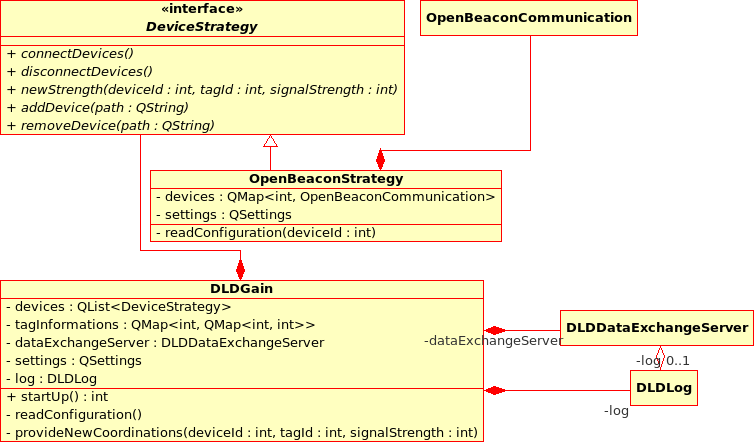
\includegraphics[scale=0.55]{UMLDiagrams/dldGainNew.png}
    \caption{UML class diagram of the adjusted gain data daemon}
    \label{fg:implementation:newGainDataDaemon}
   \end{staticFigure}

   To accelerate the development of the project the implementation of the SSL data exchange strategy was not done in this stage. Only the implementation of the D-Bus exchange strategy was performed. The implementation of the SSL exchange strategy will be done when the project has some spare time at the end. The only implementations made for SSL are the method headers to test if the communication strategy design is functional.

   \subsubsection*{Code changes that were made}
    During the implementation of the D-Bus strategy the complexity of the design was not easy to implement and due to advancement of the project the planned design was reverted to an earlier version. The current version of the design has both the server and the client in one class. With this design one signal or method would be used for both directions. One of the early versions had two classes one for the server methods and one for the client methods. This old design is now the current design to speed up the development.

  \subsection{Hardware Simulator}
   The hardware simulator was implemented to simulate and test the different daemons and applications. The drawn representation of the values was made to visualise it for the user who is testing. Right now it is reduced to only support three nodes, so only 2D position detection is supported. The hardware simulator is integrated in the data gain daemon and works as a strategy for the device backend. The extra time that was spent in the design stage to design a strategy pattern around the different hardware backends was not vain. The pure implementation as a new strategy did not take much time because of the well structured design.

  \subsection{Generate position daemon}
   The first part (receiving the signals from the data gain daemon) was done to fullfil the requirements for the distance measurement. The D-Bus Client was implemented and tested with the data gain daemon.

   \subsubsection*{Code changes that were made}
    Again the D-Bus system worked in a different way than expected. Instead of the possibility to register each object that should be accesible through D-Bus by its own only all or no Object could be added. Therefore the class for providing the different types of the position data was split up into two classes. One for the strength position and one for the relative position data calculated by this deamon.\\

    \begin{staticFigure}
     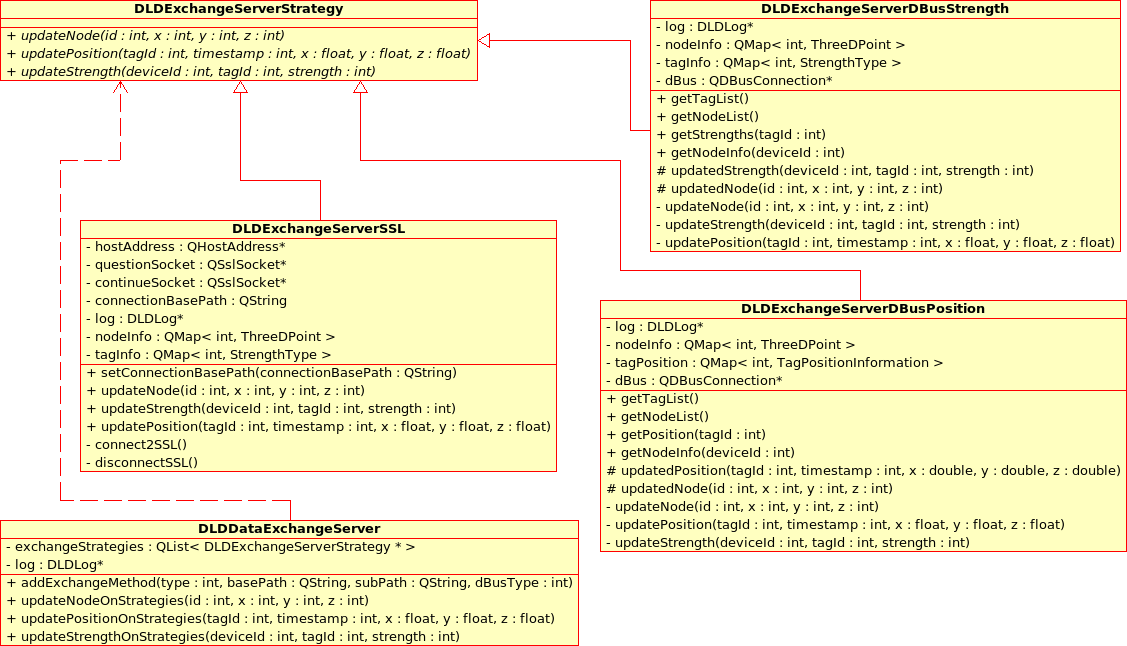
\includegraphics[scale=0.36]{UMLDiagrams/dldDataExchangeServerNew.png}
     \caption{UML class diagram of the adjusted data exchange server}
     \label{fg:implementation:newDataExchangeServer}
    \end{staticFigure}
    \begin{staticFigure}
     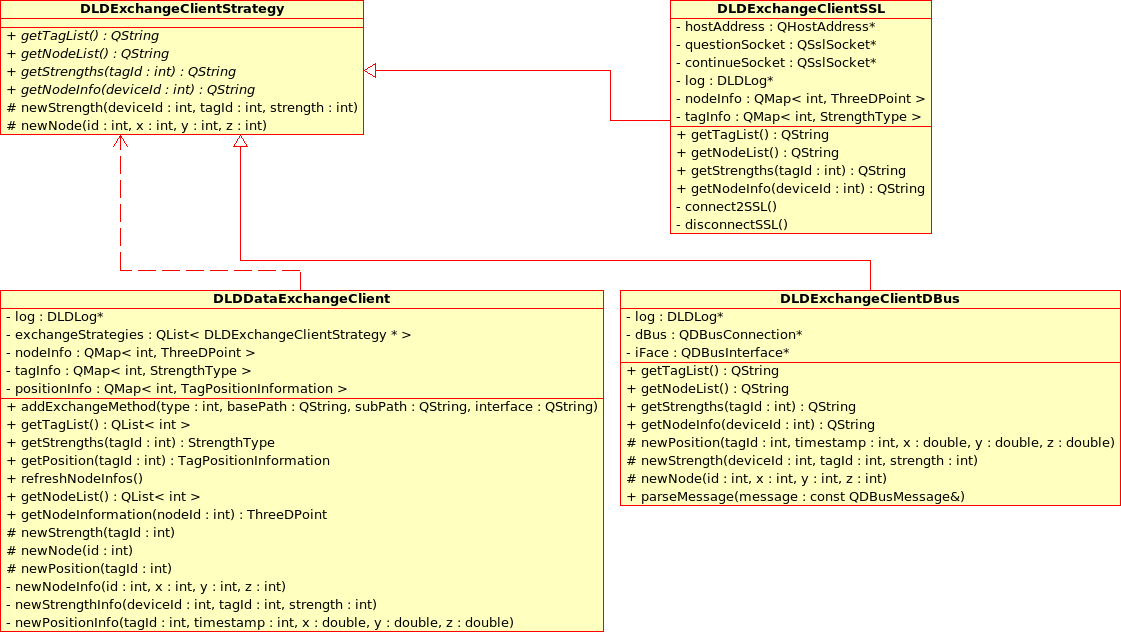
\includegraphics[scale=0.36]{UMLDiagrams/dldDataExchangeClientNew.png}
     \caption{UML class diagram of the adjusted data exchange client}
     \label{fg:implementation:newDataExchangeClient}
    \end{staticFigure}

   \subsubsection*{Changes affecting the whole project}
    Not only the D-Bus must be changed, but also the need of measurement data was reverted. The whole position localisation can be realized with only the relative data from the OpenBeacons. The maps and everything just needs to use the raw data which is generated and calculated by this daemon just on the basis of the raw packet loss. Therefore the system will look like shown in figure \ref{fg:implementation:newProjectStructure}.
    \begin{center}
     \begin{staticFigure}
      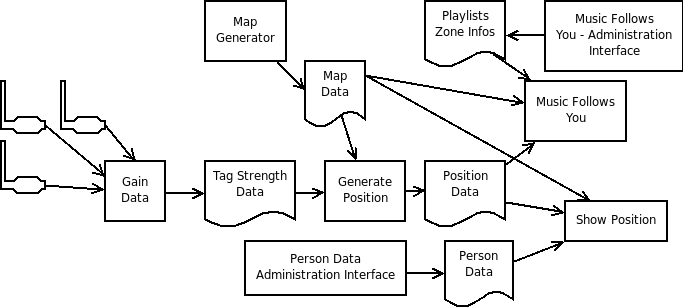
\includegraphics[scale=0.60]{Diagrams/projectStructureNew.png}
      \caption{Diagram of the adjusted project structure}
      \label{fg:implementation:newProjectStructure}
     \end{staticFigure}
    \end{center}
    
   \subsubsection*{Problems that occured during the development}
    While the RFID system worked good when only one node was used (for testing of the hardware and its performance), working with three devices at once the tag gets confused and does not send all the data back to each node. You can see that on the strength data the nodes are receiving. If two nodes are on the same axis and only one unit is between them the deviation may have a maximum of one unit. But the data that is received in some tests differs in about 5 units which means that one circle is part of the other one. This whole problem results in the fact that RFID in this constellation (based on packet loss) and with this hardware (USB OpenBeacon nodes and the active RFID tag) is unusable right now. But for the whole project this means nothing because it was planned to be used for multiple technologies, so if someone wants to create a location detection based on another hardware (WLAN for example) then only the device strategy for it must be implemented and not the whole system.

  \subsection{Administrate person data}
  \label{sec:implementation:pdAdmin}
   The implementation of the person data administration tool went straight forward and did not encounter any major problems. First the user interface was designed with the Qt designer and afterwards the functionalities of the buttons and the GUI were implemented step by step. During the implementation the example database was created too. For this purpose the database web interface phpmyadmin was used to create a database, a table and a user which can access this database. Listing \ref{lst:mysqlCommands} shows which command needs to be performed to create the example database, with all the needed information regarding the table and the user.
   \begin{lstlisting}[frame=single,breaklines,basicstyle=\footnotesize,numbers=left,label=lst:mysqlCommands,captionpos=b,caption={MySQL commands for creating the example database}]
CREATE DATABASE `dldPersons` ;

CREATE TABLE `dldPersons`.`persons` (
`tagId` INT NOT NULL ,
`name` VARCHAR( 255 ) NOT NULL ,
`prename` VARCHAR( 255 ) NOT NULL ,
`color` VARCHAR( 7 ) NOT NULL DEFAULT '#000000',
`picture` BLOB NULL ,
`description` VARCHAR( 1024 ) NULL ,
PRIMARY KEY ( `tagId` )
) ENGINE = MYISAM

CREATE USER 'dldUser'@'%' IDENTIFIED BY 'dldPass';

GRANT USAGE ON * . * TO 'dldUser'@'%' IDENTIFIED BY 'dldPass' WITH
MAX_QUERIES_PER_HOUR 0 MAX_CONNECTIONS_PER_HOUR 0 MAX_UPDATES_PER_HOUR 0
MAX_USER_CONNECTIONS 0 ;

GRANT SELECT , INSERT , UPDATE , DELETE , CREATE , INDEX , ALTER ON
`dldPersons` . * TO 'dldUser'@'%';
   \end{lstlisting}

  \subsection{Show position}
   Because of the changes that were made in the generate position daemon the show position daemon just shows the position information in a coordinate system which is relative to the received data from the nodes. After the implementation of the person data administrator was done a lot of code could be reused or copied and slightly changed for the show position daemon. In addition to the show position application a part of the planned map class and the whole map scene class were implemented. The map scene class is used to display the map data in a Qt style scene, therefore it was needed to fully implement it. The implemented part of the map class consists off all functionalities to store the most important parts. Designs like the one that is used for saving or loading maps were not implemented because they would only make sense if there was an implemented map generator. So the implementation was reduced to the minimum of functionalities plus some extra fancy stuff to make it interesting.
